\documentclass[conference]{IEEEtran}
\IEEEoverridecommandlockouts
\makeatletter
\newcommand*{\rom}[1]{\expandafter\@slowromancap\romannumeral #1@}
\makeatother
% The preceding line is only needed to identify funding in the first footnote. If that is unneeded, please comment it out.
\usepackage{cite}
\usepackage{amsmath,amssymb,amsfonts}
\usepackage{algorithmic}
\usepackage{algorithm}
\usepackage{algpseudocode}
\usepackage{graphicx}
\usepackage{textcomp}
\usepackage{multirow}
\usepackage{xcolor}
\def\BibTeX{{\rm B\kern-.05em{\sc i\kern-.025em b}\kern-.08em
    T\kern-.1667em\lower.7ex\hbox{E}\kern-.125emX}}
\begin{document}

\title{Unsupervised Domain Adaptation for RGB-D Object Recognition\\
}
\thanks{Code is available in https://github.com/amine-bs/Jigsaw-puzzle-for-RGB-D-domain-adaptation}

\author{\IEEEauthorblockN{Mohamed Amine Ben Salha}
\IEEEauthorblockA{\textit{Student} \\
\textit{Politecnico di Torino}\\
}
\and
\IEEEauthorblockN{Slim Jbeli}
\IEEEauthorblockA{\textit{Student} \\
\textit{Politecnico di Torino}\\
}
}

\maketitle

\begin{abstract}
Domain adaptation for RGB object recognition has been extensively studied and has reached very remarkable recognition levels, thanks to convolutional neural networks and different adaptation methods. In contrast, studies for domain adaptation for RGB-D inter-modal object recognition are limited and relatively new. In this paper, we study a novel RGB-D method that reduces the domain shift by exploiting the inter-modal relation between the RGB and depth image. The method consists of training a convolutional neural network to solve two tasks: the main recognition task and a pretext task.
We studied three different pretext tasks: relative rotation prediction between the RGB and depth image, relative tiles permutation prediction and absolute tiles permutation prediction. The two latter tasks are inspired by the Jigsaw puzzle unsupervised domain adaptation for RGB object recognition. We show that that relative rotation and relative permutation have similar results whereas absolute permutation have a slightly lower performance.
\\
\end{abstract}

\begin{IEEEkeywords}
Recognition, Inter-modal, Unsupervised, Adaptation
\end{IEEEkeywords}

\section{Introduction}
RGB-D data gained much importance in different domains and mainly in robotics. That’s why RGB-D object recognition became one of the main challenges. \\
Another major challenge is training algorithms.
Since supervised machine learning became the key to solve object recognition, the availability of ground-truth labels has been a major practical problem because of their cost. Therefore, methods that aim to reduce human labeling have become a major topic of research. 
Under this scope, we find many different concepts like domain generalization and self-supervised learning.
\\
In domain generalization, a model is trained to perform a prediction task in a specific domain. However, it is also required to preform the task in another correlated but different domain. The challenge here is to transfer the learned knowledge from one domain to another one that is different.
\\
In self-supervised learning, the focus is on learning features without the need for human labeling. Instead, an auxiliary simple task known as pretext task is used to train the network. The labels for this task are created automatically. This allows to train a feature extractor that will be used next to apply the main task.
\\

The main idea is to use self-supervised learning to perform domain adaptation.\\

Our goals are:
\begin{itemize}
    \item Implement some self-supervised leanring methods to achieve Domain generalization
    \item Perform hyperparameter tuning\
    \item Compare the results of the implemented methods
\end{itemize}



\section{Related work}
\subsection{Self-supervised learning}
The recent work of self-supervised learning mainly focus on the design of pretext tasks. In \cite{b1}, a pretext task of predicting the relative rotation was proposed. The labels are four possible image rotation angles that are automatically created. Another pretext task proposed in \cite{b6} consists of solving a jigsaw puzzle obtained by shuffling the tiles of an image.  

\subsection{Domain Adaptation}
The goal of domain adaptation is to achieve a good performance across multiple data distributions. The general setting consists of having a fully labeled  dataset from a source domain and  an unlabeled dataset from a different target domain. The main challenge is to learn an efficient system that transfers the knowledge from the source domain to the target domain while achieving a good performance. Many recent works address this challenge for computer vision tasks. 
\\
There have been numerous domain adaptation methods proposed for object recognition. Among the existing methods, some try to align domains at input level, like GAN based methods \cite{b3}. Some focus at feature level adaptation \cite{b4} and others on adapting the output space \cite{b5}. In \cite{b6}, the self-supervised learning method jigsaw puzzle is used for object recognition domain generalization. 
Reference \cite{b7} makes use of predicting rotation angles as pretext task to achieve domain adaptation for RGB-D datasets. 
\newline
In this work, we apply self-supervised learning to ahieve domain generalization across two different RGB-D datasets.

\section{Method}
In this section, we explain our method for RGB-D domain adaptation. Section \rom{3}-A describes the architecture of the neural network. Section \rom{3}-B provides a description of the different pretext tasks and their configurations. 

\subsection{Network architecture}
We use two different residual neural networks as feature extractors, one network for each modality. The RGB and depth features are then concatenated and given as input for the next layers. Source domain features are fed to a classification network to perform the main task. Features from both domains are fed to another network that performs the pretext task,  achieving domain adaptation. The loss function used for object recognition and the pretext task is the cross-entropy loss.
We also use entropy loss minimization which has been proved to improve the performance of unsupervised domain adaptation.


\begin{algorithm}
\caption{Unsupervised Domain Adaptation}\label{alg:cap}
\begin{algorithmic}
\textbf{Input :} 
\newline
Labeled source dataset: $S={(x^{rgb}, x^{d}, y)}$
\newline
Unlabeled target dataset: $T={(x^{rgb}, x^d)}$
\newline
\textbf{Procedure: Training the network}
\newline
$\Tilde{S}=Transform(S)$
\newline
$\Tilde{T}=Transform(T)$
\newline
\FOR{each iteration}
\newline
Load minibatch from S
\newline
Compute main loss $L_m$
\newline
Load minibatches from $\Tilde{S}$ and $\Tilde{T}$
\newline
Compute entropy minimization loss $L_e$
\newline
Compute pretext task loss $L_p$
\newline
Compute total loss $L=L_m + \lambda_e * L_e + \lambda_p * L_p$
\newline
Backpropagate total loss L
\ENDFOR

\end{algorithmic}
\end{algorithm}

\begin{figure*}[h]
\centerline{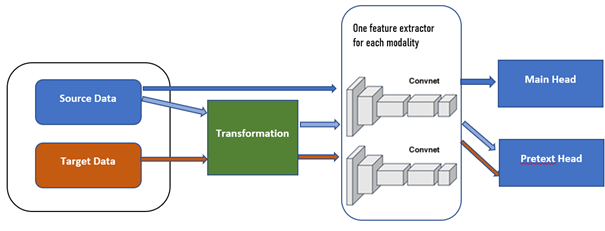
\includegraphics[width=0.7\textwidth]{network.png}}
\caption{Rotation transformation. Two different rotations are applied to each modality image.}
\label{fig}
\end{figure*}



\subsection{Pretext tasks}
Three different pretext tasks are studied in this work.

\paragraph{Relative Rotation} In this configuration, we apply a random rotation to both the RGB and depth images. The pretext task consists of predicting the relative rotation angle between the two modalities. Rotation angles are a multiple of 90° such that the output dimension of the pretext task network is 4. 

\begin{figure}[htbp]
\centerline{\includegraphics[width=0.35\textwidth]{Rotation.png}}
\caption{Rotation transformation. Two different rotations are applied to each modality image.}
\label{fig}
\end{figure}

\paragraph{Absolute Jigsaw puzzle}
In this configuration, we first split the image to a set of tiles according to a n*m grid, where n and m are hyperparameters. The next step is to randomly choose to either permute the tiles of the RGB or depth image. Finally, we apply the permutation to the chosen modality. The set of permutations is a subset of the symmetric group of n*m, $S_{n*m}$. Its cardinal is a hyperparameter and it always contains the identity permutation (which leaves the image as it is).

\begin{figure}[htbp]
\centerline{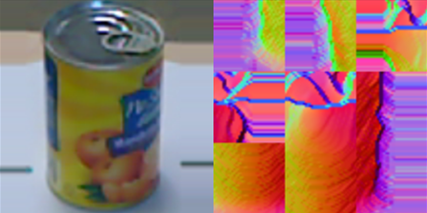
\includegraphics[width=0.35\textwidth]{absolute.png}}
\caption{Absolute Jigsaw transformation. The permutation was applied only to the depth image.}
\label{fig}
\end{figure}

\paragraph{Relative Jigsaw puzzle}
In this Setting, we apply the same first steps as in Absolute Jigsaw puzzle. However, we apply two permutations for both the tiles of the RGB and depth images. The pretext task is to predict the permutation index that superimposes the tiles of the depth image with the tiles of the RGB image. 
\newpage
In the following, we prove that the set of permutations must have the algebraic structure of a group:

Let E be the set of permutations. Solving the pretext task can be rewritten as the following statement: ($\forall f \in E, \forall g \in E$ ( $\exists!h \in E$  ($f \circ h=g$))). \\
\begin{itemize}
\item By construction, the indentity function is an element of E. 
\item Next, if we set the function g to be the identity, we prove that the inverse of each permutation in E also belongs to E. 
\item Finally, manipulating the statement proves that a combination of any two permutations is also an element of E. 
\end{itemize}
The three above characteristics show that E is a subgroup of the symmetric group $S_{n*m}$. This puts constraints on the cardinal of the permutations set and makes its construction considerably more complicated. Infact, the cardinal of a subgroup must be a divider of the cardinal of the group (that is n*m in our case). And even then, the existence of a subgroup that has a divider as a cardinal is not trivial and is hard to prove.

\begin{figure}[htbp]
\centerline{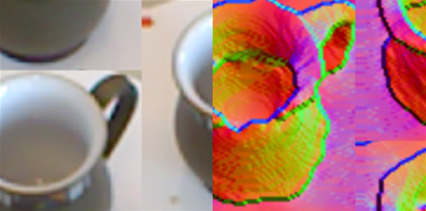
\includegraphics[width=0.35\textwidth]{relative.png}}
\caption{Relative Jigsaw transformation. Two different permutations were applied to each modality image.}
\label{fig}
\end{figure}






\section{Experiments}
\subsection{Dataset}
We use ROD and SynRod datasets to train the model. ROD is made of 41,877 RGB-D images of 51 object classes. SynROD is a synthetic dataset created using the same object models as ROD. It also contains about 41,000 RGB-D images to match the dimension of ROD. In our framework, SynROD is considered as the source domain whereas ROD is considered as the target domain.

\subsection{Implementation}
\subsubsection{Network}
The network used as a feature extractor is a pretrained ResNet-18 on ImageNet. It has proved to work well for different computer vision tasks. \\
The main task head is made of three layers: the first is a global average pooling layer, the second is a fully connected layer with 1000 neurons and the last one is also a fully connected layer with C neurons, C being the number of labels in the dataset. \\
The pretext task head is a network made of 4 layers: the first is a 2D convolutional layer with kernel size 1*1 and 100 neurons, the second layer is also a 2D convolutional layer with kernel size 3*3 and 100 neurons, the third layer is a fully connected layer with 100 neurons and the final layer is a fully connected layer with P neurons, P being the label dimension of the pretext task.\\
All convolutional and fully connected layers use batch normalization and ReLU activation function, except for the output layers which use softmax activation function.

\subsubsection{Optimization}
The weights of the main and pretext heads are initialized with Xavier initialization. The network is trained using SGD optimizer with momentum 0.9. The weight of entropy-minimization loss is 0.1 throughout all the experiments. We also include a dropout of value 0.5. The weight of the pretext task loss is 0.7. 
\subsection{Results}
In this section, we describe the obtained results. The first part consists mainly of showing the results for a set of different hyperparameters. The second section consists of comparing the performance of the different pretext tasks.
\subsubsection{Hyperparameter tuning}

\begin{table}[htbp]
\caption{Baseline target accuracy, batch size 32}
\begin{center}
\begin{tabular}{cc|c|c|c|}
\cline{3-4}
& & \multicolumn{2}{ c| }{Weight decay} \\ 
\cline{3-4}
& & 0.05 & 0.005  \\ 
\hline
\multicolumn{1}{ |c  }{\multirow{2}{*}{learning rate} } &
\multicolumn{1}{ |c| }{0.003} & 0.1031 & 0.1352   \\ 
\cline{2-4}
\multicolumn{1}{ |c  }{}                        &
\multicolumn{1}{ |c| }{0.0003} & 0.2050 & 0.3852    \\ 
\hline
\end{tabular}
\end{center}
\end{table}

\begin{table}[htbp]
\caption{Baseline target accuracy, batch size 64}
\begin{center}
\begin{tabular}{cc|c|c|c|}
\cline{3-4}
& & \multicolumn{2}{ c| }{Weight decay} \\ 
\cline{3-4}
& & 0.05 & 0.005  \\ 
\hline
\multicolumn{1}{ |c  }{\multirow{2}{*}{Learning rate} } &
\multicolumn{1}{ |c| }{0.003} & 0.2117 & 0.3351  \\ 
\cline{2-4}
\multicolumn{1}{ |c  }{}                        &
\multicolumn{1}{ |c| }{0.0003} & 0.23 & 0.4256    \\ 
\hline
\end{tabular}
\end{center}
\end{table}

\begin{table}[htbp]
\caption{Target accuracy using relative rotation DA}
\begin{center}
\begin{tabular}{cc|c|c|c|}
\cline{3-4}
& & \multicolumn{2}{ c| }{Weight decay} \\ 
\cline{3-4}
& & 0.05 & 0.005  \\ 
\hline
\multicolumn{1}{ |c  }{\multirow{2}{*}{Learning rate} } &
\multicolumn{1}{ |c| }{0.003} & 0.2396 & 0.6085    \\ 
\cline{2-4}
\multicolumn{1}{ |c  }{}                        &
\multicolumn{1}{ |c| }{0.0003} & 0.6047 & 0.6403     \\ 
\hline

\end{tabular}
\end{center}
\end{table}

\begin{table}[htbp]
\caption{Target accuracy using Absolute Jigsaw DA}
\begin{center}
\begin{tabular}{cc|c|c|c|}
\cline{3-4}
& & \multicolumn{2}{ c| }{Grid size} \\ 
\cline{3-4}
& & 3*3 & 6*5  \\ 
\hline
\multicolumn{1}{ |c  }{\multirow{2}{*}{Number of permutations} } &
\multicolumn{1}{ |c| }{9} & 0.6012 & 0.5405    \\ 
\cline{2-4}
\multicolumn{1}{ |c  }{}                        &
\multicolumn{1}{ |c| }{30} & 0.6440 & 0.5927     \\ 
\hline

\end{tabular}
\end{center}
\end{table}

\begin{table}[htbp]
\caption{Target accuracy using Relative Jigsaw DA}
\begin{center}
\begin{tabular}{cc|c|c|c|}
\cline{3-4}
& & \multicolumn{2}{ c| }{Grid size} \\ 
\cline{3-4}
& & 3*3 & 6*5  \\ 
\hline
\multicolumn{1}{ |c  }{\multirow{2}{*}{Number of permutations} } &
\multicolumn{1}{ |c| }{9} & 0.6395 & \textbf{-}    \\ 
\cline{2-4}
\multicolumn{1}{ |c  }{}                        &
\multicolumn{1}{ |c| }{30} & \textbf{-} & 0.6274     \\ 
\hline

\end{tabular}
\end{center}
\end{table}

We started by tuning the hyperparameters on the baseline model. All the reported results are obtained by training the models for 20 epochs. Tables [1] and [2] show that a batch size of 32 yields a remarkably lower performance than a batch size of 64. Thus we decided to set the batch size to 64 for the rest of experiments. \\
We inducted a cross-validation on the weight decay and the learning rate values for both the baseline and the relative rotation models. Since the same network architecture was used for all the pretext tasks, we only considered the cross validation on the relative rotation model. According to table table [3], a weight decay of 0.005 and a learning rate of 0.0003 yield the best performance. Therefore, we used these values for the rest of experiments.
Tables 4 and 5 report the target accuracy using relative and absolute jigsaw puzzle solving for different grid sizes and different numbers of permutations. 


\subsubsection{Discussion}
We find that all the methods achieve better accuracy on the target domain, compared to the baseline model.
\\
From tables 4 and 5, we conclude that the grid size and the number of permutations are critical for the Jigsaw Domain Adaptation. The most relevant grid size is 3*3 and the most relevant number of permutations is 30. 
\\
We find that the relative Jigsaw puzzle setting achieves a  2\% higher accuracy compared to the absolute Jigsaw puzzle, when using the same hyperparameters.
However, as it was mentioned previously, in the relative Jigsaw puzzle setting, the number of permutations cannot be an arbitrary integer. 
\section{Conclusion}
In this work, we have explored self-supervised learning for domain generalization for RGB-D data. We have studied several pretext tasks as domain adaptation strategies. Taking object recognition as a main task, we compared the different performances achieved by the pretext tasks. As a future work, we would like to develop the relative jigsaw puzzle strategy by constructing more permutation sets with different cardinals.




\begin{thebibliography}{00}
\bibitem{b1} Spyros Gidaris, Praveer Singh, Nikos Komodakis, ``Unsupervised Representation Learning by Predicting Image Rotations,'' in ICLR 2018.
\bibitem{b3} J. Hoffman, E. Tzeng, T. Park, J.-Y. Zhu, P. Isola, K. Saenko, A. A. Efros, and T. Darrell, “Cycada: Cycle consistent adversarial domain adaptation,” in ICML, 2018.
\bibitem{b4} Z. Pei, Z. Cao, M. Long, and J. Wang, “Multi-adversarial domain adaptation,” in AAAI, 2018.
\bibitem{b5} K. Saito, K. Watanabe, Y. Ushiku, and T. Harada, “Maximum classifier discrepancy for unsupervised domain adaptation,” in CVPR, 2018.
\bibitem{b6} Fabio Maria Carlucci, Antonio D'Innocente, Silvia Bucci, Barbara Caputo, Tatiana Tommasi, ``Domain Generalization by Solving Jigsaw Puzzles,'' in CVPR 2019.
\bibitem{b7} Mohammad Reza Loghmani, Luca Robbiano, Mirco Planamente, Kiru Park, Barbara Caputo and Markus Vincze, ``Unsupervised Domain Adaptation through Inter-modal Rotation for RGB-D Object Recognition,'' in CVPR 2019.
\end{thebibliography}


\end{document}
